\documentclass{comjnl}
\usepackage[utf8x]{inputenc}
\usepackage{amsmath}
\usepackage{graphicx}

%% These two lines are needed to get the correct paper size
%% in TeX Live 2016
\let\pdfpageheight\paperheight
\let\pdfpagewidth\paperwidth

%\copyrightyear{2009} \vol{00} \issue{0} \DOI{000}

\begin{document}
\title[Physiopathologie de la sclerose en plaque]{
\includegraphics[scale=0.09]{logo.png} \\ Physiopathologie de la sclerose en plaque}
\author{Julien DENOZI}
\affiliation{Master 1 Bioinformatique, Connaissance et Donnees, Problematique et Structures en Sante, Faculte des Sciences de Montpellier } \email{denozi.j@gmail.com}

\shortauthors{Physiopathologie de la sclerose en plaque}
 



%\category{C.2}{Computer Communication Networks}{Computer Networks}
%\category{C.4}{Performance of Systems}{Analytical Models}
%\category{G.3}{Stochastic Processes}{Queueing Systems}
%\terms{Internet Technologies, E-Commerce}



\begin{abstract}
La sclérose en plaque (SEP) est une maladie auto-immune qui touche des individus prédisposés génétiquement, mais qui semble être déclenchés par des facteurs environnementaux. La maladie cause des lésions sur les gaines de myélines altérant ainsi la capacité du système nerveux à communiquer  et ainsi provoquer de nombreux symptômes physiques et mentaux.

\end{abstract}

\maketitle


\section{Introduction}
La sclérose en plaque est une pathologie du système nerveux centrale caractérisé par des lésions des gaînes de myélines disséminés spatialement induisant des symptomes et déficit multiples et variées.
Le plus souvent la maladie évolue par poussées, au cours desquelles les symptômes apparaissent et disparaissent continuellement. Au bout d’un certain nombre d’année ces poussées laissent place à des séquelles qui peuvent se révéler très invalidantes altérant ainsi le contrôle des mouvements, la perception sensorielle, la mémoire, la parole etc...
La sclérose en plaque se décline quatre formes évolutives:
\begin{enumerate}
\item Forme récurrente-rémittente (SEP RR)= cycle de crise et de rémissions.
\item Forme progressive secondaire (SEP PR)=progression graduelle de la maladie avec un cycle de rémissions et de rechute.
\item Forme progressive primaire (SEP PP)=évolution de la maladie de manière progressive sans rémissions et peut s’arrêter temporairement.
\item Forme récurrente-progressive(SEP RP)=évolution de la maladie de manière progressive sans arrêt et sans rémissions.
\end{enumerate}



\section{Symptomatologie}
Etant la première cause de handicap non traumatique chez les sujets jeunes et affectant plus de 90 000 patients en France, cette maladie fait son apparition entre 20 et 40 ans.
Les inflammations étant disséminés dans l'espace et le temps sont la cause de nombreux symptômes variés allant du trouble de la vision, de la motricité, de la sensibilité ou encore de l'humeur. Ces caractéristiques correspondent toutes à une atteinte du système nerveux central et sont le socle sur lequelle le diagnostique peut être effectuer.
\begin{figure*}[h!]
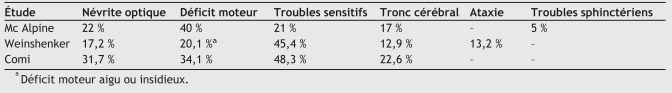
\includegraphics[width=1 \textwidth]{signe_inauguraux.png}
\caption{Tableaux Récapitulatif des signes inauguraux de personnes atteintes de la sclérose en plaque \cite{Ouallet2004}}
\end{figure*}

\subsection{Signe clinique }
Lors de l'examen clinique de nombreux symptômes/signes sont révélateurs d'une sclérose en plaque:
\begin{enumerate}
\item Le syndrome pyramidale se manisfestant par un trouble de la marche avec une asthénie chronique.
\item Le signe de Babinski correspondant à une extension des orteils lors de la stimulation de la voûte plantaire.
\item La névrite optique se manifestant par une baisse de l'acuité visuelle, des douleurs occulaires et orbitaires ainsi qu'une atrophie de la papille optique signe d'une atteinte du nerf optique.
\item des troubles de la sensibilité: paresthésie, sensation de décharge dans le rachis lors de la flexion du cou, anesthésie des récepteurs thermo-algésique.
\item Des vertige, nystagmus et ataxie.
\item Le syndrome cérébelleux correspondant à une atteinte du cervelet causant une difficulté à la station debout et une marche asynchronée.
\item La paralysie faciale

\end{enumerate}
Les lésions provoqués par la SEP sont s'y disséminer, qu'elles peuvent provoquer un panel de signes/symptôme très grands. La liste s'y dessus ne se veut pas exhaustive, mais permet de montrer l'étendu des lésions que peuvent provoquer la SEP.

\subsection{Examen complémentaire}
L'imagerie par résonnance magnétique (IRM) constitue le meilleur moyen de déceler une SEP, en effet cette examen permet de réaliser des coupes dont l'orientation est totalement aux choix de l'examinateur et par conséquent permet de retrouver une zone très blanche autour des ventricules cérébraux caractéristiques. Cependant il est a noter que la plupart du temps ces lésions sont asymptomatiques et plus vieilles, le sujet jeune se voit assez fréquemment pourvues de ces lésions. Le critère déterminant est donc l'association d'accident neurologique et de la présence de lésions jeunes ( mise en évidence par du gadolinum).

 \begin{figure}[h!]
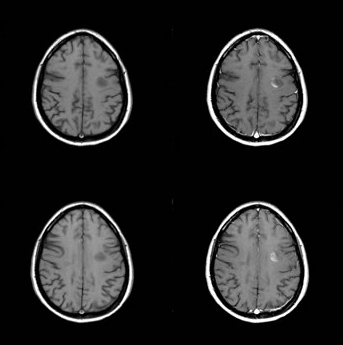
\includegraphics[width=0.4\textwidth]{irm1.png}
\caption{Imagerie par résonnance magnétique avant injection de produit de contraste}
\end{figure}

\section{Ethiopathogénie}
L’étiopathogénie de cette maladie n’est pas encore connu, c’est pour cette raison qu’elle est au centre de nombreuses recherches qui visent à comprendre les raisons de l’apparition de cette maladie.
Il a été clairement admis que les causes sont multiples et relèvent de caractères génétiques comme environnementaux, ainsi des expositions à des agents chimiques, modes de nutrition ou encore au temps d’exposition de l’individu au soleil constituent des des explications potentielles de la contraction de la maladie.
Plusieurs études ont permis de mettre en relation la participation des gène en relation avec le système immunitaire, et des gènes qui ne sont pas en relation initialement avec le système immunitaire.
Ainsi plusieurs techniques sont mis en oeuvre comme les puces à ADN qui permettent l’identification de nouveaux gènes impliqués dans l’apparition de la sclérose en plaque ou encore Ribo Tag  permettant d’isoler des ARNm spécifiques.
Les nombreuses études réalisés ont permit d'établir la prévalence de la SEP dans de nombreux pays,en majorités industrialisés. Ainsi nous retrouvons environs 20 à 200 cas pour 100 000 habitants.
\subsection{Approche génétique}
Selon Compston \cite{Compston2005}  le risque de développer un SEP est de 1/600 pour un Européen,1/200 pour un enfant née d'un parent atteint d'une SEP, 1/40 pour le frère ou la soeur ( ou du jumeau dizygote) d'un sujet atteint de la SEP et 1/13 pour le jumeau monozygote.
Malgré les avancées scientifiques et technologique aucun gène majeur n'a pu être mis en évidence.

\subsection{Approche virale et bactériologique }
De nombreuses idées soutiennent que les facteurs environnementaux jouent un rôle dans le déclenchement de la SEP, cependant aucun agent infectieux n'a été identifié à ce jours bien que la présence de certain anticorps situé dans le liquide céphalo-rachidien soit souvent retrouvés chez les patients atteind de la SEP (rougeole, rubéole, Epstein-Barr, HSV2, oreillon).
Ainsi l'implication d'un seul agent infectieux commun à tout les cas de SEP est très peu probable.
A contrario, il est possible que l'exposition du système immunitaire à certains agents infectieux durant l'enfance jouent un rôle de protection dans la contraction de la SEP \cite{Bach2002}

\section{Thérapeutiques}
\subsection{Traitement symptomatiques}
La rééducation neurologiques contribuent à :
\begin{enumerate}
\item Préserver l'autonomie de la marche, la station debout et les activités quotidiennes.
\item Prévenir les escares chez les patients ayant une mobilité très réduite.
\end{enumerate}


\bibliographystyle{acm}
\bibliography{collection}


\end{document}